\chapter{实验思路}

\section{目录格式}

\textbf{目录标题}:三号宋体,加粗,居中,段前20磅,段后10磅,无缩进,“目”和“录”之间空4格;

\textbf{各章题序及其余}:小4号宋体;自动生成,段前段后0磅;一级标题空2个字符(空4格),二级标题空4个字符(空8格),三级标题空6个字符(空12格)。

上述格式已经在模板中正确定义。

\section{正文格式}

\subsection{正文标题}

论文正文分章节撰写,每章开始另起一页书写。各章标题要突出重点、简明扼要。字数一般应在15字以内,不加标点符号。

各级标题理科顶格。

\begin{enumerate}
    \item 章标题四号加粗,多倍行距值1.25,段前20磅,段后10磅。
    \item 节标题小四号加粗,多倍行距值1.25,段前0.5行,段后0.5行。
    \item 条标题五号加粗,多倍行距值1.25,段前0.5行,段后0.5行。
    \item 款、项标题五号,多倍行距值1.25,段前0行,段后0行。
\end{enumerate}

上述格式要求中,章、节、条已经根据具体格式要求作了定义,请分别使用\texttt{\textbackslash chapter}、\texttt{\textbackslash section}和\texttt{\textbackslash subsection}。对于款、项标题,并未作区分,均使用\texttt{\textbackslash subsubsection}。

\subsection{正文文本}

正文中所用字体,一律中文字体为宋体,数字、英文为新罗马字体。正文采用小四号,多倍行距值1.25,段前0行,段后0行,首行缩进2个字符。

\section{引用文献标注}

\subsection{引用文献标注格式}

引文标注采用顺序编码制。正文中引用文献的标示应置于所引内容最后一个字的右上角,所引文献编号用阿拉伯数字置于方括号“[ ]”中,用小4号字体的上角标。

由于此处引文未作详细要求,因此在本模板中直接采用2015年的国标文件中定义的引用格式,符合实验报告要求中有关引文格式的要求。

\subsection{使用BIB管理引用文献}

模板使用\texttt{biblatex}管理参考文献格式。在引用文献之前,需要首先在\texttt{*.bib}文件中定义参考文献条目,随后使用\texttt{\textbackslash cite\{key\}}命令插入引用。如下代码框\ref{lst:bib}展示了一个引用文献的BIB条目:

\begin{lstlisting}[caption={BIB引文格式条目示例\label{lst:bib}}]
@article{demo,
  author = {袁庆龙 and 候文义},
  journal = {太原理工大学学报},
  number = {32(1)},
  title = {Ni-P合金镀层组织形貌及显微硬度研究},
  volume = {51-53},
  year = {2001}
}
\end{lstlisting}

这句话展示了一篇文献引用的示例\cite{demo}。

\section{插入公式}

对于公式,实验报告的要求是论文中的公式应另起行,若公式前有文字(如“解”、“假定”等),文字前空4个字符。公式应标注序号,并将序号置于括号内。序号按章编排,如第一章第一个公式的序号为“(1.1)”。文中引用公式时,一般用“见式(1.1)”或“由公式(1.1)”。公式末不加标点符号。公式应该是可编辑的,若是采用word2007版编写的公式,在文档转化为2003版之后,公式会转化为图片,应该再用2003的office版本重新编辑。公式段前段后3磅,1.25倍行距。公式主体居中,序号右对齐。作者可以根据实际情况调整,保持美观。

对于包含“假定”或“解”字样的公式,模板提供了\texttt{\textbackslash prefacedEqu}命令的实现,参考式(\ref{equ:assumption})的示例。

\prefacedEqu{假定}{\label{equ:assumption} X \sim N(\mu, \sigma)}

式(\ref{equ:assumption})对应的\TeX 源码如代码\ref{lst:tex_source_code}所示。

\begin{lstlisting}[
  language=tex, 
  caption={式(\ref{equ:assumption})对应的\TeX 源码\label{lst:tex_source_code}}]
\prefacedEqu{假定}{\label{equ:assumption} X \sim N(\mu, \sigma)}
\end{lstlisting}

方法通过在字样后使用负值的\texttt{\textbackslash vspace\{\}}强行把字样压到与公式平齐的方法实现,接受两个参数:公式前的字样;和一个选项:公式前字样强行下降的高度(用于以防命令在某些情况下字样下降高度不符合实际要求的时候能够根据情况手动调整),在不给出选项值的情况下字样将默认下降值相当于\texttt{\textbackslash baselineskip}的高度。

由于是通过暴力压高度的方法实现的,因此使用\texttt{\textbackslash prefacedEqu}命令对公式长度有限制要求。使用该命令时请勤换行公式,参照式(\ref{equ:longequ})所示的编写方式。

\prefacedEqu{解}{\label{equ:longequ}
  \begin{aligned}
    & \int e^{2x} \arctan \sqrt{e^x - 1} \mathrm{d} x \\
    & \xRightarrow{\mathrm{Integration\ by\ Parts}}
        \dfrac{1}{2} \int \arctan \sqrt{ e^x - 1 }
            \mathrm{d} \left(e^{2x}\right) \\
    & = \dfrac{e^{2x}}{2} \cdot \arctan \sqrt{ e^x - 1 }
        - \dfrac{1}{2} \int e^{2x} \cdot \dfrac{1}{1 + e^x -1} \cdot \dfrac{1}{2 \sqrt{e^x -1}} \mathrm{d} x \\ 
    & = \dfrac{e^{2x} \arctan \sqrt{ e^x - 1 }}{2}
        - \dfrac{1}{4} \int \dfrac{e^{2x}}{\sqrt{ e^x - 1 }} \mathrm{d}x
  \end{aligned}
}

\section{插入表格}

插表之前文中必须有相关文字提示,如“见表1.1”、“如表1.1所示”。

这里推荐大家在Excel中使用Excel2TeX宏插件实现将Excel转为表格形式,插入的学术三线表如表\ref{tab:demo}所示。

% Table generated by Excel2LaTeX from sheet 'Sheet1'
\begin{table}[htbp]
  \centering
  \caption{单位在每列的书写示例}\label{tab:demo}
    \begin{tabular}{crlrr}
    \toprule
    \multicolumn{1}{l}{基体} & \multicolumn{1}{l}{序号} & 粉末类型和预热温度(℃) & \multicolumn{1}{l}{失效温度(℃)} & \multicolumn{1}{l}{Ec计算值(GPa)} \\
    \midrule
    \multirow{4}[2]{*}{SUS304不锈钢} & 1     & 粗粉\& 1000 & 180   & 4.21 \\
          & 2     & 粗粉\& 800 & 10    & 4.38 \\
          & 3     & 细粉\& 1000 & 300   & 4.95 \\
          & 4     & 细粉\& 800 & 120   & 5.08 \\
    \bottomrule
    \end{tabular}%
  \label{tab:addlabel}%
\end{table}%  

根据格式要求,一般情况下插表不能拆开两页编排,如某表在一页内安排不下时,才可转页,以续表形式接排,表左上角注明编号,编号后加“(续表)”,并重复表头。

为了解决上述要求,模板提供了如下的三个命令以便用户能够从容应对长表格编写的难题:

\begin{enumerate}
    \item \texttt{\textbackslash getlongtablecols} ——用于获取表格的列数;
    \item \texttt{\textbackslash storecaption} ——将文本保存为一个变量,随后插入为表格的caption及多次调用;
    \item \texttt{\textbackslash mycaption} ——使用过\texttt{\textbackslash storecaption}将一段文本保存标题变量之后使用\texttt{\textbackslash mycaption}可以调用保存的标题文本内容;
    \item \texttt{\textbackslash continuetablephrase} ——插入续表的表头,在longtable环境中置于\texttt{\textbackslash endfirsthead} 与 \texttt{\textbackslash endhead}之间。
\end{enumerate}

上述命令请具体参照表\ref{tab:long}中的示例,展示了一张跨越多页的长表格\cite{2024lnmcm}。

% Table generated by Excel2LaTeX from sheet 'Sheet1'
		\begin{longtable}{ccccccc}
      \storecaption{插入长表格并自动适配表标题的示例}\\
			\caption{\mycaption} \label{tab:long} \\
			
			\toprule 带钢厚度  & 带钢宽度  & 碳含量   & 硅含量   & 带钢速度  & 加热炉温度 & 均热炉温度 \\ \midrule 
			\endfirsthead
			
			\continuetablephrase \\
			\toprule 带钢厚度  & 带钢宽度  & 碳含量   & 硅含量   & 带钢速度  & 加热炉温度 & 均热炉温度 \\ \midrule 
			\endhead
			
			\bottomrule
			\endfoot
			
			\bottomrule
			\endlastfoot
      8450  & 193   & 299   & 8     & 549   & 732.8 & 688.5 \\
      8320  & 192   & 353   & 7     & 549   & 747.8 & 710.5 \\
      8290  & 232   & 343   & 6     & 580   & 715.2 & 635.5 \\
      8360  & 201   & 411   & 15    & 649   & 717.2 & 650 \\
      8880  & 223   & 376   & 6     & 609   & 711.4 & 634 \\
      8360  & 202   & 337   & 6     & 600   & 732.8 & 650.5 \\
      8120  & 234   & 353   & 5     & 679   & 751.2 & 643 \\
      8440  & 203   & 395   & 8     & 481   & 683.6 & 634 \\
      8120  & 234   & 442   & 8     & 649   & 743.2 & 641 \\
      8360  & 203   & 417   & 10    & 649   & 714.8 & 638.5 \\
      8350  & 201   & 374   & 7     & 667   & 725.8 & 652.5 \\
      8620  & 182   & 351   & 6     & 649   & 698.8 & 634 \\
      8360  & 201   & 440   & 11    & 679   & 730.6 & 650 \\
      8640  & 224   & 507   & 9     & 590   & 697.8 & 634.5 \\
      8960  & 202   & 373   & 12    & 552   & 693.8 & 645 \\
      9150  & 193   & 438   & 7     & 600   & 700   & 636 \\
      8140  & 231   & 400   & 8     & 599   & 724.4 & 645 \\
      8350  & 202   & 361   & 6     & 649   & 729   & 652 \\
      8620  & 182   & 410   & 7     & 648   & 699.8 & 631 \\
      8960  & 203   & 383   & 11    & 563   & 698.6 & 634 \\
      8020  & 225   & 360   & 8     & 549   & 733.6 & 643 \\
      8360  & 192   & 419   & 11    & 649   & 711.2 & 646.5 \\
      9360  & 202   & 384   & 10    & 606   & 730.6 & 645 \\
      8700  & 201   & 352   & 7     & 679   & 732.2 & 654.5 \\
      8360  & 202   & 382   & 8     & 649   & 734.8 & 658.5 \\
      8960  & 203   & 422   & 7     & 649   & 730   & 636 \\
      8300  & 214   & 403   & 6     & 648   & 710.8 & 630 \\
      8440  & 193   & 367   & 9     & 629   & 729.2 & 656 \\
      8170  & 191   & 357   & 12    & 599   & 714.2 & 652.5 \\
      8770  & 181   & 360   & 7     & 528   & 690.8 & 653 \\
      8720  & 192   & 436   & 9     & 555   & 701.4 & 641.5 \\
      8960  & 202   & 358   & 9     & 590   & 705.4 & 648.5 \\
      8700  & 202   & 443   & 7     & 649   & 720.4 & 637.5 \\
      9570  & 222   & 430   & 11    & 628   & 727.2 & 640.5 \\
      8420  & 202   & 353   & 8     & 648   & 717   & 644 \\
      8370  & 201   & 441   & 14    & 630   & 716.6 & 664 \\
      8720  & 203   & 300   & 8     & 540   & 737.6 & 692.5 \\
      8360  & 202   & 385   & 8     & 649   & 734.2 & 658.5 \\
      8700  & 201   & 352   & 7     & 649   & 720   & 648.5 \\
      9220  & 202   & 413   & 7     & 569   & 706   & 638.5 \\
      8700  & 202   & 425   & 9     & 581   & 714   & 643.5 \\
      8960  & 203   & 372   & 8     & 620   & 705.4 & 642 \\
      8370  & 201   & 347   & 7     & 649   & 720   & 658.5 \\
      8960  & 203   & 414   & 8     & 500   & 679   & 620.5 \\
      8820  & 223   & 271   & 6     & 618   & 791.2 & 719.5 \\
      9380  & 182   & 406   & 9     & 600   & 689.6 & 635 \\
\end{longtable}

\section{插入图片}

\subsection{总体要求}

根据格式要求:插图应与文字紧密配合,文图相符,内容正确。选图要精练,插图、照片应完整清晰。

\subsection{图题及图中说明}

每个图均应有图题(由图序和图名组成),居中位置。图题不宜有标点符号。图名在图序之后空1个字符排写。图序按章编排,如第l章第一个插图的图号为“图1.1”,第2章第一个插图的图号为“图2.1”等。图题置于图下,只需用中文书写,有图注或其它说明时应置于图题之上。引用图应注明出处,在图题右上角加引用文献号。

上述格式要求在模板中已有完整的定义。这里用户无需再对图标题格式作额外的修改,直接插入图片方式就能满足格式的要求。

图中若有分图时,分图题置于分图之下或图题之下,分图号用a)、b)等表示。图题用5号加粗,段前段后0行,1.25倍行距。图中文字和数字等字号用5号字体。

考虑到以往的\texttt{subfigure}宏包已不再维护,模板将默认使用更加现代的\texttt{subcaption}宏包。图\ref{fig:figures}展示了一个基本的分图示例,其中具体的分图如分图\ref{fig:a}和分图\ref{fig:b}所示。

\begin{figure}[!h]
  \centering
  \begin{minipage}{0.4\linewidth}
    \centering
    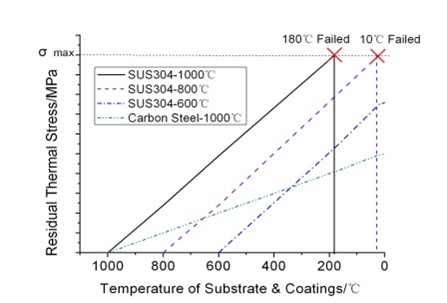
\includegraphics[
      height=0.2\textheight
      ]{figure/subfig1.jpg}
      \subcaption{粗粉涂层}\label{fig:a}
  \end{minipage}
  \begin{minipage}{0.4\linewidth}
    \centering
    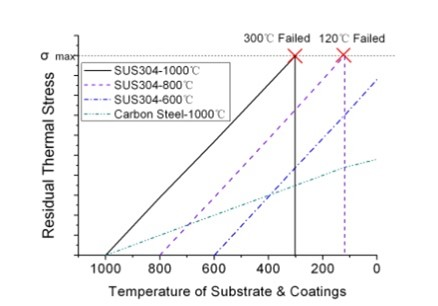
\includegraphics[
      height=0.2\textheight
      ]{figure/subfig2.jpg}
      \subcaption{细粉涂层}\label{fig:b}
  \end{minipage}
  \caption{涂层在冷却过程中残余热应力的变化情况}
  \label{fig:figures}
\end{figure}

\subsection{插图编排}

图的样式必须为嵌入式,居中。插图之前,文中必须有关于本插图的提示,如“见图1.1”、“如图1.1所示”等。插图与其图题为一个整体,不得拆开排写于两页。插图处的该页空白不够排写该图整体时,则可将其后文字部分提前排写,将图移到次页。但是全文的图的编号不能乱,图2.1必须在图2.2之前。有分图时,分图过多在一页内安排不下时,可转到下页,总图题只出现在下页。图与上下正文间需空一行编排。

\section{插入代码块}

尽管在格式要求文件中没有提及,但考虑到代码块的使用比较频繁也比较繁琐,本模板将其一并提供。在本模板中是使用\texttt{listings}宏包插入代码块的,代码块有两种调用形式:

\begin{enumerate}
  \item 在\TeX 中嵌入代码块;
  \item 或以文件形式插入代码。
\end{enumerate}

通过在\TeX 中嵌入代码的形式插入代码块的示例如\ref{lst:insert}所示。

\begin{lstlisting}[language=C, caption={在\TeX 中嵌入代码的形式插入代码块\label{lst:insert}}]
#include <stdio.h>
int main( void ) {
  print("hello, world\n");
  return 0;
}
\end{lstlisting}

以文件形式插入代码块的示例见附录代码\ref{lst:demo}。
    
\section{结论}

根据报告格式要求,“结论”项有如下的格式要求:

\textbf{结论标题}:四号宋体,加粗,顶格,段前20磅,段后10磅,1.25倍行距。

\textbf{结论内容}:宋体小四,段前段后0行,1.25倍行距。

由于上述格式要求并不明确,没有声明“结论”标题的具体位置。但此处“结论”的格式要求实际上与章标题完全一致,因此这里认为结论命令应当居于文档左侧。读者可以使用本模板提供的\texttt{\textbackslash conclusion}命令来生成符合格式要求的“结论”字样。如下展示了一个符合格式要求的“结论”行:

\conclusion

就我们目前所能测定的情况来看,花生酱对地球的自转没有什么影响\cite{PeanutButter}。
